\documentclass[dvips, lscape]{foils}
%\documentclass[dvips, french]{slides}
\textwidth 18.5cm
\textheight 25cm 
\topmargin -1cm 
\oddsidemargin  -1cm 
\evensidemargin  -1cm

% Maths
\usepackage{amsfonts, amsmath, amssymb}

\newcommand{\coefbin}[2]{\left( 
    \begin{array}{c} #1 \\ #2 \end{array} 
  \right)}
\newcommand{\Bcal}{\mathcal{B}}
\newcommand{\Ccal}{\mathcal{C}}
\newcommand{\Dcal}{\mathcal{D}}
\newcommand{\Ecal}{\mathcal{E}}
\newcommand{\Gcal}{\mathcal{G}}
\newcommand{\Mcal}{\mathcal{M}}
\newcommand{\Ncal}{\mathcal{N}}
\newcommand{\Pcal}{\mathcal{P}}
\newcommand{\Qcal}{\mathcal{Q}}
\newcommand{\Lcal}{\mathcal{L}}
\newcommand{\Tcal}{\mathcal{T}}
\newcommand{\Ucal}{\mathcal{U}}
\newcommand{\alphabf}{\mbox{\mathversion{bold}{$\alpha$}}}
\newcommand{\betabf}{\mbox{\mathversion{bold}{$\beta$}}}
\newcommand{\gammabf}{\mbox{\mathversion{bold}{$\gamma$}}}
\newcommand{\mubf}{\mbox{\mathversion{bold}{$\mu$}}}
\newcommand{\Pibf}{\mbox{\mathversion{bold}{$\Pi$}}}
\newcommand{\psibf}{\mbox{\mathversion{bold}{$\psi$}}}
\newcommand{\Thetabf}{\mbox{\mathversion{bold}{$\Theta$}}}
\newcommand{\taubf}{\mbox{\mathversion{bold}{$\tau$}}}
\newcommand{\Cbf}{{\bf C}}
\newcommand{\Ebf}{{\bf E}}
\newcommand{\Gbf}{{\bf G}}
\newcommand{\Hbf}{{\bf H}}
\newcommand{\Ibf}{{\bf I}}
\newcommand{\mbf}{{\bf m}}
\newcommand{\Rbf}{{\bf R}}
\newcommand{\Sbf}{{\bf S}}
\newcommand{\Tbf}{{\bf T}}
\newcommand{\ubf}{{\bf u}}
\newcommand{\Ubf}{{\bf U}}
\newcommand{\vbf}{{\bf v}}
\newcommand{\Vbf}{{\bf V}}
\newcommand{\xbf}{{\bf x}}
\newcommand{\Xbf}{{\bf X}}
\newcommand{\Ybf}{{\bf Y}}
\newcommand{\Zbf}{{\bf Z}}
\newcommand{\Esp}{{\mathbb E}}
\newcommand{\Var}{{\mathbb V}}
\newcommand{\Cov}{{\mathbb C}\mbox{ov}}
\newcommand{\Ibb}{{\mathbb I}}
\newcommand{\Rbb}{\mathbb{R}}

% sommes
\newcommand{\sumk}{\sum_k}
\newcommand{\sumt}{\sum_{t \in I_k}}
\newcommand{\sumth}{\sum_{t=t_{k-1}^{(h)}+1}^{t_k^{(h)}}}
\newcommand{\sump}{\sum_{p=1}^{P}}
\newcommand{\suml}{\sum_{\ell=1}^{P}}
\newcommand{\sumtau}{\sum_k \widehat{\tau}_{kp}}

% Couleur et graphiques
\usepackage{color}
\usepackage{graphics}
\usepackage{epsfig} 
\usepackage{pstcol}

% Texte
\usepackage{lscape}
\usepackage{../../../../Latex/fancyheadings, rotating, enumerate}
%\usepackage[french]{babel}
\usepackage[latin1]{inputenc}
\definecolor{darkgreen}{cmyk}{0.5, 0, 0.5, 0.5}
\definecolor{orange}{cmyk}{0, 0.6, 0.8, 0}
\definecolor{jaune}{cmyk}{0, 0.5, 0.5, 0}
\newcommand{\textblue}[1]{\textcolor{blue}{#1}}
\newcommand{\textred}[1]{\textcolor{red}{#1}}
\newcommand{\textgreen}[1]{\textcolor{green}{ #1}}
\newcommand{\textlightgreen}[1]{\textcolor{green}{#1}}
%\newcommand{\textgreen}[1]{\textcolor{darkgreen}{#1}}
\newcommand{\textorange}[1]{\textcolor{orange}{#1}}
\newcommand{\textyellow}[1]{\textcolor{yellow}{#1}}
\newcommand{\refer}[2]{\textgreen{[{\sl #1, #2}]}}
\newcommand{\emphase}[1]{\textblue{#1}}

% Sections
%\newcommand{\chapter}[1]{\centerline{\LARGE \textblue{#1}}}
% \newcommand{\section}[1]{\centerline{\Large \textblue{#1}}}
% \newcommand{\subsection}[1]{\noindent{\Large \textblue{#1}}}
% \newcommand{\subsubsection}[1]{\noindent{\large \textblue{#1}}}
% \newcommand{\paragraph}[1]{\noindent {\textblue{#1}}}
% Sectionsred
\newcommand{\chapter}[1]{
  \addtocounter{chapter}{1}
  \setcounter{section}{0}
  \setcounter{subsection}{0}
%   {\centerline{\LARGE \textblue{\arabic{chapter} - #1}}}
  {\centerline{\LARGE \textblue{#1}}}
  }
\newcommand{\section}[1]{
  \addtocounter{section}{1}
  \setcounter{subsection}{0}
%   {\centerline{\Large \textblue{\arabic{chapter}.\arabic{section} - #1}}}
%   }
  {\centerline{\Large \textblue{#1}}}
  }
\newcommand{\subsection}[1]{
  \addtocounter{subsection}{1}
  {\noindent{\large \textblue{#1}}}
  }
% \newcommand{\subsection}[1]{
%   \addtocounter{subsection}{1}
%   {\noindent{\large \textblue{\arabic{chapter}.\arabic{section}.\arabic{subsection} - #1}}}
%   }
\newcommand{\paragraph}[1]{\noindent{\textblue{#1}}}

%%%%%%%%%%%%%%%%%%%%%%%%%%%%%%%%%%%%%%%%%%%%%%%%%%%%%%%%%%%%%%%%%%%%%%
%%%%%%%%%%%%%%%%%%%%%%%%%%%%%%%%%%%%%%%%%%%%%%%%%%%%%%%%%%%%%%%%%%%%%%
%%%%%%%%%%%%%%%%%%%%%%%%%%%%%%%%%%%%%%%%%%%%%%%%%%%%%%%%%%%%%%%%%%%%%%
%%%%%%%%%%%%%%%%%%%%%%%%%%%%%%%%%%%%%%%%%%%%%%%%%%%%%%%%%%%%%%%%%%%%%%
\begin{document}
%%%%%%%%%%%%%%%%%%%%%%%%%%%%%%%%%%%%%%%%%%%%%%%%%%%%%%%%%%%%%%%%%%%%%%
%%%%%%%%%%%%%%%%%%%%%%%%%%%%%%%%%%%%%%%%%%%%%%%%%%%%%%%%%%%%%%%%%%%%%%
%%%%%%%%%%%%%%%%%%%%%%%%%%%%%%%%%%%%%%%%%%%%%%%%%%%%%%%%%%%%%%%%%%%%%%
%%%%%%%%%%%%%%%%%%%%%%%%%%%%%%%%%%%%%%%%%%%%%%%%%%%%%%%%%%%%%%%%%%%%%%
\landscape
\newcounter{chapter}
\newcounter{section}
\newcounter{subsection}
\setcounter{chapter}{0}
\headrulewidth 0pt 
\pagestyle{fancy} 
\cfoot{}
\rfoot{\begin{rotate}{90}{
      \hspace{1cm} \tiny Statistical analysis of CGH data
      }\end{rotate}}
\rhead{\begin{rotate}{90}{
      \hspace{-.5cm} \tiny \thepage
      }\end{rotate}}

%%%%%%%%%%%%%%%%%%%%%%%%%%%%%%%%%%%%%%%%%%%%%%%%%%%%%%%%%%%%%%%%%%%%%%
%%%%%%%%%%%%%%%%%%%%%%%%%%%%%%%%%%%%%%%%%%%%%%%%%%%%%%%%%%%%%%%%%%%%%%
\begin{center}
  \textblue{\LARGE Statistical Analysis of CGH Arrays}

   \vspace{1cm}
   {\large E. Lebarbier, S. Robin, B. Thiam} \\
   robin@agroparistech.fr
   
   {UMR AgroParisTech / INRA: Math�matique et Informatique Appliqu�es}
   \\
   {SSB group: genome.jouy.inra.fr/ssb/}
   
    \vspace{1cm}
    { R�union AgriArray } \\
    {Montpellier, 13 - 12 - 2007}
\end{center}

%\vspace{2cm}
\paragraph{Outline} \\
\\
\begin{tabular}{lcl}
  1 - Principle of CGH array analysis
  & & 3 -  Multiple arrays analysis\\ 
  \\
  2 - Looking for breakpoints
  & & 4 - Segment classification \\
\end{tabular}


%%%%%%%%%%%%%%%%%%%%%%%%%%%%%%%%%%%%%%%%%%%%%%%%%%%%%%%%%%%%%
%%%%%%%%%%%%%%%%%%%%%%%%%%%%%%%%%%%%%%%%%%%%%%%%%%%%%%%%%%%%%
\newpage
\chapter{Principle of CGH array analysis}
%%%%%%%%%%%%%%%%%%%%%%%%%%%%%%%%%%%%%%%%%%%%%%%%%%%%%%%%%%%%%
%%%%%%%%%%%%%%%%%%%%%%%%%%%%%%%%%%%%%%%%%%%%%%%%%%%%%%%%%%%%%

\vspace{-1cm}
$$
\epsfig{file = ../Figures/principe_CGH.eps, clip=,
  bbllx=0, bblly=41, bburx=700, bbury=478, scale=0.9}
$$

%%%%%%%%%%%%%%%%%%%%%%%%%%%%%%%%%%%%%%%%%%%%%%%%%%%%%%%%%%%%%
\newpage
\section{Interpretation of a CGH profile }
%%%%%%%%%%%%%%%%%%%%%%%%%%%%%%%%%%%%%%%%%%%%%%%%%%%%%%%%%%%%%

\noindent
\begin{tabular}{cc}
  \begin{tabular}{p{7cm}}
    \paragraph{Data size.} \\
    \\
    Few thousands points / genome\\
    \\
    Few hundreds points / chromosome\\
    \\ \\ \\ \\
    \paragraph{A dot on the graph = }
  \end{tabular} 
  &
  \begin{tabular}{c}
    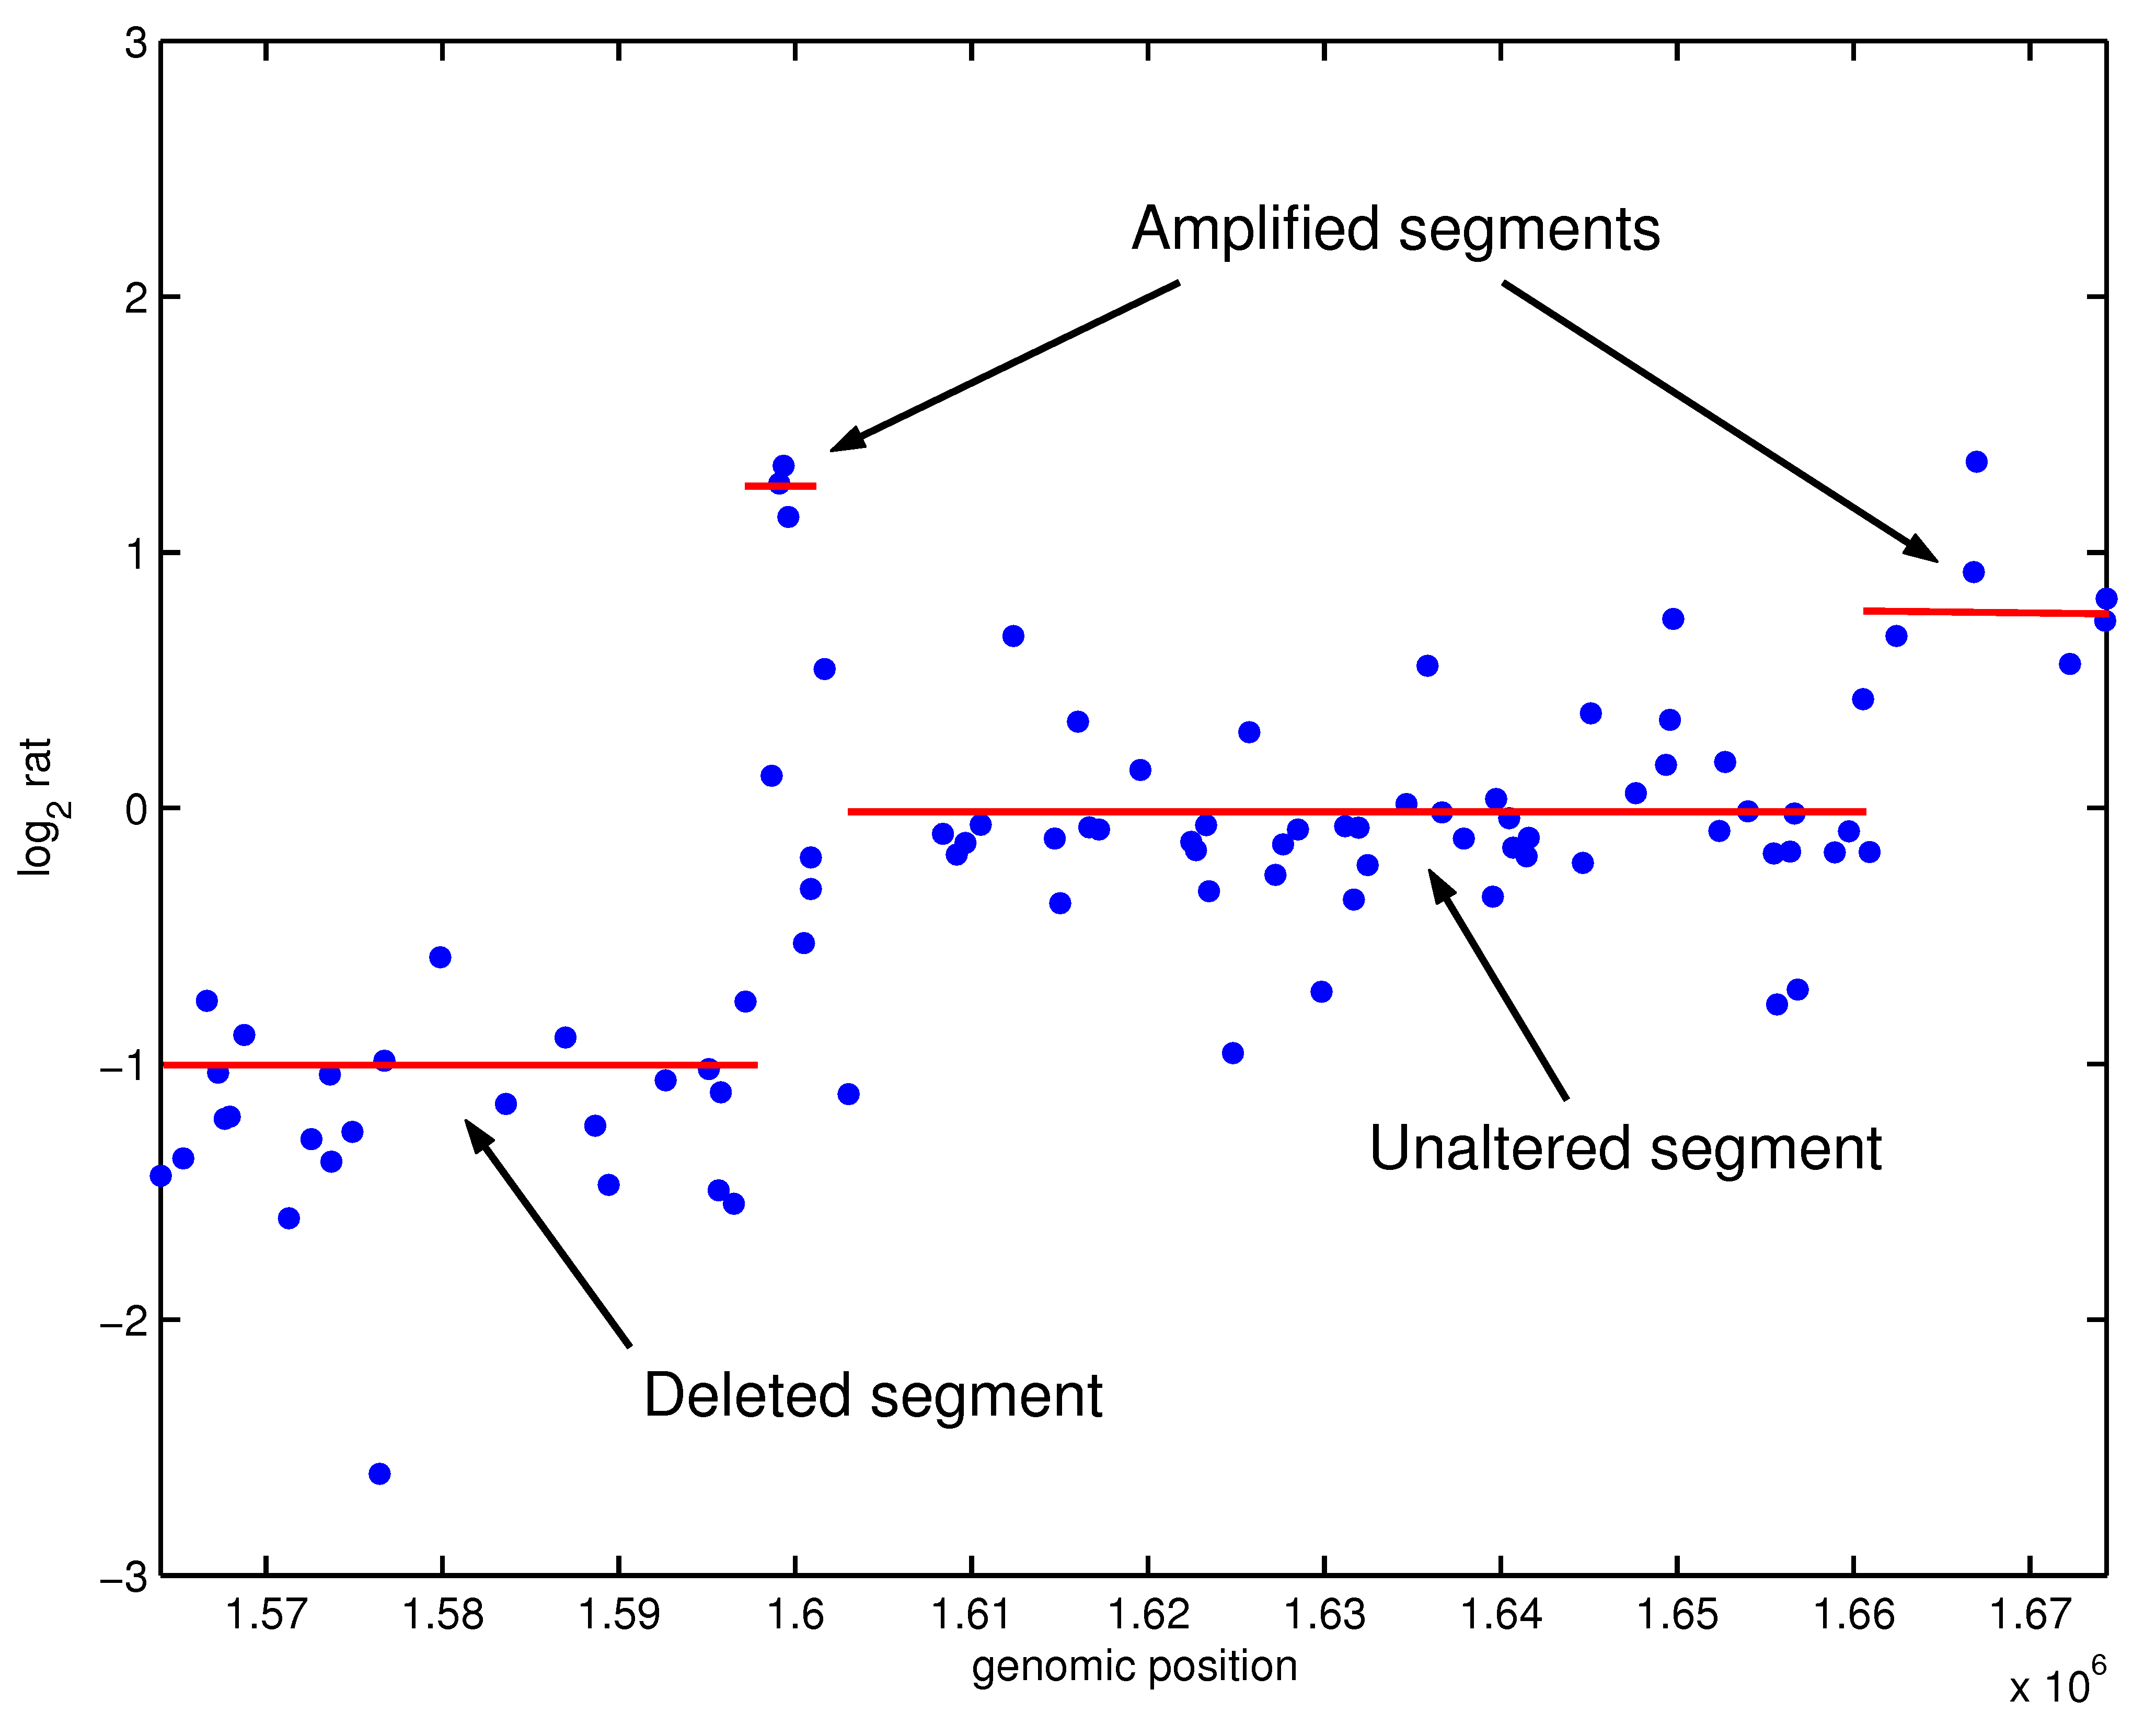
\epsfig{file = ../Figures/profile_example.eps, clip=,
      bbllx=60, bblly=196, bburx=543, bbury=586, width=16cm}
  \end{tabular} 
\end{tabular} 
\vspace{-0.25cm}
$$
\log_2 \left\{ \frac{\text{ $\sharp$ copies of BAC(t) in the test
      genome }}{\text{$\sharp$ copies of BAC(t) in the reference
      genome}}\right\}
$$


%%%%%%%%%%%%%%%%%%%%%%%%%%%%%%%%%%%%%%%%%%%%%%%%%%%%%%%%%%%%%
%%%%%%%%%%%%%%%%%%%%%%%%%%%%%%%%%%%%%%%%%%%%%%%%%%%%%%%%%%%%%
\newpage
\chapter{Looking for breakpoints}
%%%%%%%%%%%%%%%%%%%%%%%%%%%%%%%%%%%%%%%%%%%%%%%%%%%%%%%%%%%%%
%%%%%%%%%%%%%%%%%%%%%%%%%%%%%%%%%%%%%%%%%%%%%%%%%%%%%%%%%%%%%

%%%%%%%%%%%%%%%%%%%%%%%%%%%%%%%%%%%%%%%%%%%%%%%%%%%%%%%%%%
\bigskip
%\section{What to we have in mind?}
\section{Statistical model} 
%%%%%%%%%%%%%%%%%%%%%%%%%%%%%%%%%%%%%%%%%%%%%%%%%%%%%%%%%%

\begin{itemize}
\item At position $t$, there exists a 'true' log-ratio, which depends
  on the relative copy number.
\item The value of the true log-ratio is affected by abrupt changes:
                                %\vspace{-0.5cm}
  $$
  \epsfig{file = ../Figures/FigSeg_Intro_ter.eps, clip=, bbllx=90,
    bblly=300, bburx=540, bbury=400, scale = 1.2}
  $$
  Positions \emphase{$t_1$, $t_2$, ..} are called
  \emphase{breakpoints}. \emphase{$\mu_k$} is the true log-ratio in
  segment \emphase{$I_k$}.
\item The observed signal $Y_t$ is noisy:
  $$
  \mbox{if } t \in I_k: 
  \qquad Y_t \sim \Ncal(\mu_k, \sigma^2_{(k)}), 
  \qquad \{Y_t\}_t \mbox{ independent}.
  $$
\end{itemize}
%   where $\lambda_t$ is the true log-ratio 
%   and $E_t$ is a noise (typically, $E_t \sim \Ncal(0, \sigma^2)$).


% %%%%%%%%%%%%%%%%%%%%%%%%%%%%%%%%%%%%%%%%%%%%%%%%%%%%%%%%%%
% \newpage
% \section{Statistical model} 
% %%%%%%%%%%%%%%%%%%%%%%%%%%%%%%%%%%%%%%%%%%%%%%%%%%%%%%%%%%
% \vspace{-0.5cm}\begin{itemize}
% \item The breakpoints define a partition of the data into $K$
%   segments of size $n_k$:
%   $$
%   I_k=\{t, t \in ]t_{k-1},t_k]\}, 
%   \qquad
%   Y^k=\{Y_t, t \in I_k\}.
%   $$
% \item Suppose that these parameters are constant between two changes
%   \refer{Picard et al.}{2005}: 
%   $$
%   \mbox{if position $t$ is in segments $I_k$,} \qquad Y_t = \mu_k +
%   E_t \sim \Ncal(\mu_k,\sigma_{(k)}^2).
%   $$
% \item The parameters of this model are: 
%   $$
%   T  =  (t_1, ..., t_{K-1}),
%   \qquad
%   \Theta  = (\theta_1,\hdots,\theta_K), \quad \theta_k=(\mu_k,\sigma_{(k)}^2).
%   $$
% \end{itemize}
% Breakpoints detection aims at studying the \textblue{spatial structure
%   of the signal}.

%%%%%%%%%%%%%%%%%%%%%%%%%%%%%%%%%%%%%%%%%%%%%%%%%%%%%%%%%%
\newpage
\subsection{How to find the breakpoints?}

When the number of segments $K$ is known , we have to minimize
$$
J_k(1, n) = \sum_{k=1}^K \sum_{t \in I_k} (Y_t - \widehat{\mu}_k)^2.
$$
\begin{itemize}
\item The $\coefbin{n-1}{K-1}$ possible choices for the positions of
  the breakpoints $t_1, t_2, \dots, t_{K-1}$ can not be explored for
  large $n$ and $K$
\item $\sum_{t \in I_k} (Y_t - \widehat{\mu}_k)^2$ can be viewed as
  the \emphase{'cost' of segment $I_k$}, i.e. the cost of gathering
  data $Y_{t_{k-1}+1}$ to $Y_{t_{k+1}}$ into a single segment.
\item The optimization problem is actually a shortest path problem
  that can be solved thanks to \emphase{dynamic programming}
  \refer{Picard et al.}{2005}.
\end{itemize}


%%%%%%%%%%%%%%%%%%%%%%%%%%%%%%%%%%%%%%%%%%%%%%%%%%%%%%%%%%
\newpage
\subsection{One last problem: the selection of $K$}

\noindent
\begin{tabular}{cc}
  \begin{tabular}{p{10cm}}
    \begin{itemize}
    \item $J_K$ decreases when $K$ (\emphase{complexity}) increases.
    \item Standard criteria such as AIC or BIC are
      \emphase{not valid}.
    \item \emphase{Penalty function}: $pen(K) = $ $K+1$ or $2K$.
    \item We look for the minimum of
      $$
      J_k + \beta pen(K)
      $$
      where $\beta$ is given \refer{Lebarbier}{2005} or adaptively
      estimated \refer{Lavielle}{2003}.
    \end{itemize}
  \end{tabular}
  &
  \begin{tabular}{c}
    \epsfig{file = ../Figures/Select_K.ps, clip=, bbllx=146, bblly=529,
      bburx=464, bbury=777, width=12cm, height=12cm} 
  \end{tabular}
\end{tabular}

% %%%%%%%%%%%%%%%%%%%%%%%%%%%%%%%%%%%%%%%%%%%%%%%%%%%%%%%%%%
% \newpage
% \section{Example of segmentation on array CGH data}
% %%%%%%%%%%%%%%%%%%%%%%%%%%%%%%%%%%%%%%%%%%%%%%%%%%%%%%%%%%

% \paragraph{Are the variances $\sigma^2_k$ homogeneous?} BT474 cell
% line, chromosome 9: 
% $$
% \begin{tabular}{cc}
%   Homogeneous variances & Heterogeneous variances \\
%   \multicolumn{2}{c}{$K=4$ segments} \\
%   \epsfig{file = ../Figures/bt474_c9_seg_homo_K4.eps, clip=, scale=0.7} &
%   \epsfig{file = ../Figures/bt474_c9_seg_hetero_K4.eps, clip=, scale=0.7} \\
% \end{tabular}
% $$

% %%%%%%%%%%%%%%%%%%%%%%%%%%%%%%%%%%%%%%%%%%%%%%%%%%%%%%%%%%
% \newpage
% \paragraph{Adaptive choice of the number of segments.} BT474 cell
% line, chromosome 1:
% $$
% \begin{tabular}{cc}
%   Homogeneous variances & Heterogeneous variances \\
%   $\widehat{K} = 10$  segments & $\widehat{K} = 2$ segments \\
%   \epsfig{file = ../Figures/bt474_c1_seg_homo_K10.eps, clip=, scale=0.7} &
%   \epsfig{file = ../Figures/bt474_c1_seg_hetero_K2.eps, clip=, scale=0.7} \\
% \end{tabular}
% $$
% Homogeneous variances result in smaller segments.

%%%%%%%%%%%%%%%%%%%%%%%%%%%%%%%%%%%%%%%%%%%%%%%%%%%%%%%%%%
\newpage
\subsection{Comparative study} 

\vspace{-0.5cm}
\paragraph{Lai \& al. (Bioinformatics, 05).} On both synthetic and
real data (GBM brain tumor data), the dynamic programming approach
outperfoms other methods available at that time.
$$
%\epsfig{file = ../Figures/LPJ05-Fig1.eps, clip=, scale=1.2}
%\epsfig{file = ../Figures/LPJ05-Fig3.eps, clip=, scale=1.2}
\epsfig{file = ../Figures/LPJ05-Fig4.eps, clip=, scale=1.2}
$$

%%%%%%%%%%%%%%%%%%%%%%%%%%%%%%%%%%%%%%%%%%%%%%%%%%%%%%%%%%%%%
%%%%%%%%%%%%%%%%%%%%%%%%%%%%%%%%%%%%%%%%%%%%%%%%%%%%%%%%%%%%%
\newpage
\chapter{Multiple arrays analysis}
%%%%%%%%%%%%%%%%%%%%%%%%%%%%%%%%%%%%%%%%%%%%%%%%%%%%%%%%%%%%%
%%%%%%%%%%%%%%%%%%%%%%%%%%%%%%%%%%%%%%%%%%%%%%%%%%%%%%%%%%%%%

\subsection{Two examples.}

\paragraph{1 - Comparing {\sl A. Thaliana} mutants or ecotypes.}
Chromosomal rearrangement can be detected by comparing CGH profiles
observed on individual from different genotypes.

\paragraph{2 - Comparing groups of patients.}
To detect chromosomal aberration associated with a specific disease
(e.g. breast cancer), we analyse the profiles of several ill patients
jointly.

\bigskip\bigskip
\subsection{First approach: Common breakpoints.}

Assuming that all the patients of the same group have their
breakpoints at the same positions, leads to \emphase{segment a
  multivariate signal}, which can be achieved using DP.

This is doable but \emphase{biologically irrelevant}.

%%%%%%%%%%%%%%%%%%%%%%%%%%%%%%%%%%%%%%%%%%%%%%%%%%%%%%%%%%
\newpage
\subsection{Breast cancer dataset (Inst. Curie): Chromosome 8.} \\
\\
\begin{tabular}{ccc}
  & Good prognosis (53 patients) & Bad prognosis (81 patients) \\
  \hspace{-1cm}
  \begin{tabular}{p{2.5cm}} Number of breakpoints \end{tabular} &
  \begin{tabular}{c}
    \epsfig{file =
      /RECHERCHE/RUPTURES/Exposes/Figures/CurieChromo8Gp1_K.eps, clip=,
      width=10cm, height=6cm}
  \end{tabular} 
  &
  \begin{tabular}{c}
    \epsfig{file =
      /RECHERCHE/RUPTURES/Exposes/Figures/CurieChromo8Gp2_K.eps, clip=,
      width=10cm, height=6cm} 
  \end{tabular} \\
  \hspace{-1cm}
  \begin{tabular}{p{2.5cm}} Position of the breakpoints \end{tabular} &
  \begin{tabular}{c}
    \epsfig{file =
      /RECHERCHE/RUPTURES/Exposes/Figures/CurieChromo8Gp1_T.eps, clip=,
      width=10cm}
  \end{tabular} 
  &
  \begin{tabular}{c}
    \epsfig{file =
      /RECHERCHE/RUPTURES/Exposes/Figures/CurieChromo8Gp2_T.eps, clip=,
      width=10cm}
  \end{tabular} 
\end{tabular}

%%%%%%%%%%%%%%%%%%%%%%%%%%%%%%%%%%%%%%%%%%%%%%%%%%%%%%%%%%%%%
\newpage
\section{Correlated profiles}
%%%%%%%%%%%%%%%%%%%%%%%%%%%%%%%%%%%%%%%%%%%%%%%%%%%%%%%%%%%%%

\hspace{-2cm}
\begin{tabular}{cc}
  \begin{tabular}{p{12cm}}
    We want to account for \emphase{correlations between profiles}. \\ \\
    \emphase{Different probe affinities} may alter all the profiles at the same
    position. \\ \\
    Denoting $Y_{it}$ the profile of patient $i$ at position $t$
    (belonging to segment $I_{ik}$), we
    set
    $$
    Y_{it} = \mu_{ik} + U_t + E_{it}
    $$
    where $\mu_{ik}$ is the mean of segment $I_{ik}$ and
    \emphase{$U_t$ is the random effect of probe $t$}: 
    $$
    \{E_{it}\} \mbox{ iid } \Ncal(0, \sigma^2),  
    \quad
    \{U_t\} \mbox{ iid } \Ncal(0, \gamma^2).  
    $$
  \end{tabular}
  &
  \begin{tabular}{l}
    \epsfig{file = ../Figures/nakao-mat.txt-MixSeg.eps, width=11cm,
    height=14cm, bbllx=90, bblly=220, bburx=380, bbury=590, clip=}
  \end{tabular}
\end{tabular}

%%%%%%%%%%%%%%%%%%%%%%%%%%%%%%%%%%%%%%%%%%%%%%%%%%%%%%%%%%%%%
\newpage
\section{Mixed segmentation model}
%%%%%%%%%%%%%%%%%%%%%%%%%%%%%%%%%%%%%%%%%%%%%%%%%%%%%%%%%%%%%

\paragraph{Covariance between profiles.}
$$
\Cov(Y_{it}, Y_{i't'}) = \Cov(U_t + E_{it}, U_{t'} + E_{i't'}) = 
\left\{
  \begin{array}{cl}
    \gamma^2 & \mbox{if } t = t' \\
    0 & \mbox{otherwise}
  \end{array}.
\right.
$$

\paragraph{Matrix form.}
We end up with a mixed linear model with a segmentation term ($\Tbf$):
$$
\Ybf = \Tbf \mubf + \Zbf \Ubf + \Ebf
$$
where
\begin{itemize}
\item \vspace{-0.5cm} $m$ is the number of patients, $n$ is the length
  of each profile
\item \vspace{-0.5cm} $\Zbf$ is the ($nm \times n$) \emphase{design
    matrix} that gives the probe corresponding to each data point.
\item \vspace{-0.5cm} $\Ubf$ is the $n$-vector containing the random
  effects of the probes.
\end{itemize}
\vspace{-0.5cm} \refer{Lebarbier et al.}{2007}

%%%%%%%%%%%%%%%%%%%%%%%%%%%%%%%%%%%%%%%%%%%%%%%%%%%%%%%%%%
\newpage
\section{Estimation of the parameters}
%%%%%%%%%%%%%%%%%%%%%%%%%%%%%%%%%%%%%%%%%%%%%%%%%%%%%%%%%%

\paragraph{Direct maximisation.}
Due to correlations, the variance $\Var(\Ybf)$ is not diagonal, so the
log-likelihood $\Lcal(\Ybf)$ is not additive anymore $\Rightarrow$ No
dynamic programming

\subsection{A second  DP-EM algorithm} 

\vspace{-0.5cm}
The \emphase{conditional variance} of $\Ybf$ given $\Ubf$
($\Var(\Ybf|\Ubf)$) is diagonal, so DP can be used to estimate $\Tbf$
given $\Ubf$.  $\Ubf$ is seen as an unobserved. \refer{Foulley}{Lecture
  notes}

\paragraph{E step.} Calculate the conditional moments of the random
effect given the data:
$$
\widehat{\Esp}(\Ubf|\Ybf), \qquad \widehat{\Var}(\Ubf|\Ybf).
$$
\paragraph{M step.} Denoting $\widehat{\Ubf} = 
\widehat{\Esp}(\Ubf|\Ybf)$ , perform the segmentation as follows:
$$
\widehat{\Tbf \mubf} = \arg\min_{\Tbf\mubf} \|\Ybf -
{\Tbf\mubf}-\Zbf \widehat{\Ubf}\|^2.
$$
A \emphase{two-stage dynamic programming} is required to
  achieve this step for numerous patients. \refer{Picard et al.}{?}

%%%%%%%%%%%%%%%%%%%%%%%%%%%%%%%%%%%%%%%%%%%%%%%%%%%%%%%%%%
\newpage
\section{Nakao data, chromosome 20}
%%%%%%%%%%%%%%%%%%%%%%%%%%%%%%%%%%%%%%%%%%%%%%%%%%%%%%%%%%

The random effect has an influence on the detected breakpoints. 

\noindent
\begin{tabular}{cc}
  \begin{tabular}{p{10cm}}
    We find a \emphase{large negative random effect} $U_t$ has at position
    37. \\ \\
    $\rightarrow$ poor probe affinity or wrong annotation. ~\\ ~\\ 
  \end{tabular}
  &
  \begin{tabular}{l}
     \epsfig{file= ../FIGURES/Exemple_profiles67_groupe1.ps,
    width=12cm, height=7cm, 
    bbllx=120, bblly=450, bburx=480, bbury=580, 
    clip=}
  \end{tabular} \\
  \begin{tabular}{p{10cm}}
    Comparison \textred{individual} / multiple segmentation. \\
    \\
    The breakpoints detected around position 37 vanish. \\ 
  \end{tabular}
  &
  \begin{tabular}{l}
    \epsfig{file= ../FIGURES/Nakao20_group1_pos_U.ps, width=12cm,
      height=5cm, 
      bbllx=120, bblly=250, bburx=480, bbury=580, 
      clip=} 
  \end{tabular}
\end{tabular}

%%%%%%%%%%%%%%%%%%%%%%%%%%%%%%%%%%%%%%%%%%%%%%%%%%%%%%%%%%%%%
%%%%%%%%%%%%%%%%%%%%%%%%%%%%%%%%%%%%%%%%%%%%%%%%%%%%%%%%%%%%%
\newpage
\chapter{Segments classification}
%%%%%%%%%%%%%%%%%%%%%%%%%%%%%%%%%%%%%%%%%%%%%%%%%%%%%%%%%%%%%
%%%%%%%%%%%%%%%%%%%%%%%%%%%%%%%%%%%%%%%%%%%%%%%%%%%%%%%%%%%%%

\bigskip
\paragraph{Considering biologists objective and the need for a new
  model.}
$$
\begin{tabular}{cc}
  \epsfig{file = ../Figures/FigSegClas-1.eps, clip=, scale=0.7} &
  \epsfig{file = ../Figures/FigSegClas-2.eps, clip=, scale=0.7} \\
\end{tabular}
$$
We'd like segments of same type ('normal', 'deleted', amplified')
to be gathered into classes.
% $$
% \epsfig{file = ../Figures/nouveau_modele.ps, angle=270, clip=,
%   bbllx=92, bblly=47, bburx=484, bbury=828, scale=0.9}
% $$

%%%%%%%%%%%%%%%%%%%%%%%%%%%%%%%%%%%%%%%%%%%%%%%%%%%%%%%%%%
\newpage
\section{A segmentation-clustering model}
%%%%%%%%%%%%%%%%%%%%%%%%%%%%%%%%%%%%%%%%%%%%%%%%%%%%%%%%%%

\begin{itemize}
\item We suppose that there exists a \textblue{secondary unobserved
    structure} that clusters the $K$ segments into $P$ classes with
  proportions $\pi_1,...,\pi_P$:
% \item We introduce hidden variables, $Z_{kp}$ indicators of the
%   class of origin of \textblue{segment $k$}.
% \item These variables are supposed independent, with multinomial
%   distribution:
  $$
  \pi_p = \mbox{proportion of class $p$}, 
  \qquad \sum_p \pi_p=1.
%   (Z_{k1},\hdots,Z_{kP}) \sim \mathcal{M}(1;\pi_1,\hdots,\pi_P).
  $$
\item Conditionally to the class to which the segment belongs, we know
  the distribution of $Y$:
  $$
  t \in I_k, k \in p \qquad \Rightarrow \qquad Y_t \sim \Ncal(m_p, s_p^2).
%   Y^k|Z_{kp}=1 \sim \Ncal({\bf 1}_{n_k} m_p, s_p^2 {\bf I}_{n_k}).
  $$
  \refer{Picard et al.}{2007}
%\item It is a model of \textblue{segmentation/clustering}.
\end{itemize}

The parameters of this model are
\begin{eqnarray*}
  \mbox{the breakpoint positions:} & \quad & T = \{t_1, ..., t_{K-1}\} ,\\
  \mbox{the mixture characteristics:} & \quad & \Psi = (\{\pi_p\}, \{m_p\},
  \{s^2_p\}). 
\end{eqnarray*}


%%%%%%%%%%%%%%%%%%%%%%%%%%%%%%%%%%%%%%%%%%%%%%%%%%%%%%%%%%%
\newpage
\section{BT474 cell line}
%%%%%%%%%%%%%%%%%%%%%%%%%%%%%%%%%%%%%%%%%%%%%%%%%%%%%%%%%%%

\paragraph{Interest of clustering: an easy case.} Chromosome 9:
$$
  \begin{tabular}{cc}
    Segmentation & Segmentation / Clustering \\
    \multicolumn{2}{c}{$K=4$ segments} \\
    \epsfig{file = ../Figures/bt474_c9_seg_homo_K4, clip=, scale=0.7} 
    & 
    \epsfig{file = ../Figures/bt474_c9_segclas_homo_P3K4 , clip=, scale=0.7} 
  \end{tabular}
$$
Clustering defines 'deleted', 'normal' and 'amplified' classes.

\newpage

\paragraph{Interest of clustering: a more interesting case.}
Chromosome 1:
$$
\begin{tabular}{cc}
  Segmentation & Segmentation / Clustering \\
  $K=2$ & $P=3$, $K=8$ \\
  \epsfig{file = ../Figures/bt474_c1_seg_hetero_K2.eps, clip=, scale=0.7} 
  & \epsfig{file = ../Figures/resultat_P3K8.eps , clip=, scale=0.7} 
\end{tabular}
$$
Clustering detects an outliers and captures a 'normal' segment within
a large variance region.


%%%%%%%%%%%%%%%%%%%%%%%%%%%%%%%%%%%%%%%%%%%%%%%%%%%%%%%%%%%%%%%%%%%%%%
%%%%%%%%%%%%%%%%%%%%%%%%%%%%%%%%%%%%%%%%%%%%%%%%%%%%%%%%%%%%%%%%%%%%%%
%%%%%%%%%%%%%%%%%%%%%%%%%%%%%%%%%%%%%%%%%%%%%%%%%%%%%%%%%%%%%%%%%%%%%%
%%%%%%%%%%%%%%%%%%%%%%%%%%%%%%%%%%%%%%%%%%%%%%%%%%%%%%%%%%%%%%%%%%%%%%
\end{document}
%%%%%%%%%%%%%%%%%%%%%%%%%%%%%%%%%%%%%%%%%%%%%%%%%%%%%%%%%%%%%%%%%%%%%%
%%%%%%%%%%%%%%%%%%%%%%%%%%%%%%%%%%%%%%%%%%%%%%%%%%%%%%%%%%%%%%%%%%%%%%
%%%%%%%%%%%%%%%%%%%%%%%%%%%%%%%%%%%%%%%%%%%%%%%%%%%%%%%%%%%%%%%%%%%%%%
%%%%%%%%%%%%%%%%%%%%%%%%%%%%%%%%%%%%%%%%%%%%%%%%%%%%%%%%%%%%%%%%%%%%%%
